\section{Elastic Media and Waves}
    Internal forces that resemble the force in Hooke's law lead to wave motion. This means that if $h(x, t)$ is some variation from equilibrium (one dimension but could be generalized to $\va{r}$) then the variable $h$ must satisfy the wave equation. 
    \begin{equation*}
        \pdv[2]{h}{x} = \frac{1}{v^2} \pdv[2]{h}{t}
    \end{equation*}
    This equation arises from applying Newton's second law to the elastic medium. This equation is linear so any linear combination of two known solutions is also a solution (\textbf{superposition principle}). $v$ is the \textbf{wave speed} and is $$v = \sqrt{\frac{\text{restoring force factor}}{\text{inertial factor}}}$$
    The solution to the wave equation is $h(x, t) = g(x - vt)$ for any function $g$. $h$ is a \textbf{traveling wave}, and it represents some shape described by $g$ moving in the $x$-direction with velocity $v$. If g takes a sinusoidal form, h is a \textbf{harmonic wave}.
    \begin{equation*}
        h(x, t)= H\sin(k(x - vt)) = H\sin(kx - \omega t)
    \end{equation*}
    $H$ is the \textbf{amplitude}, the maximum departure from equilibrium. $k$ and $\omega$ the repeat length and time. The \textbf{wavelength} $\lambda$ (repeat length), \textbf{period} $T$, and frequency $f = 1 / T$ are specified by the \textbf{wave number} $k$ and \textbf{angular frequency} $\omega$. 
    \begin{equation*}
        \omega = 2\pi f = \frac{2\pi}{T} \text{ and } k = \frac{2\pi}{\lambda}
    \end{equation*}
    and wave speed links wavelength and frequency.
    \begin{equation*}
        v = \lambda f
    \end{equation*}
    Fourier's theorem states that any wave can be written as a linear combination of harmonic waves.
    \newline \indent
    Another solution for the wave equation is for \textbf{standing waves}, with an equation
    \begin{equation*}
        h(x, t) = H\sin(kx + \varphi)\cos (\omega t + \delta)
    \end{equation*}
    These waves oscillate in place rather than traveling. Frequency is still $f = \omega / 2\pi$. The wavelength is given by $\lambda = 2L / n$ where $n$ is the number of nodes minus 1.
    \newline \indent
    Waves can either be \textbf{transverse} (the displacement is perpendicular to the motion of the wave),
    \begin{center}
        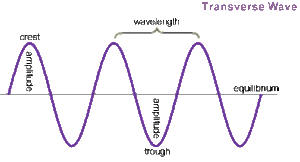
\includegraphics[width=70pt]{transverse.png}
    \end{center}
    or \textbf{longitudinal} (the displacement is parallel to the motion of the wave).
    \begin{center}
        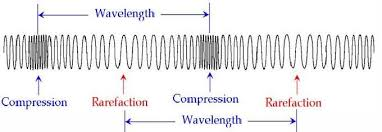
\includegraphics[width=70pt]{longitudinal.jpg}
    \end{center}
    \subsection*{Power and Energy in Waves}
        The \textbf{power} of a wave is the rate at which energy is delivered through a unit area perpendicular to the waves motion. For a harmonic wave propagating on a string of mass density $\mu$,
        \begin{equation*}
            P = \mu v \omega^2 H^2 \cos^2(kx - \omega t)
        \end{equation*}
        The energy density in the harmonic wave is $P / v$. Both power and energy density are both traveling waves as well and are proportional to the amplitude squared and the frequency squared.
    \subsection*{Reflection and Refraction}
        Waves that reach boundaries between different media reflect back into the original medium and refract into the new one. The refracted wave is called the \textbf{transmitted} wave. The amplitudes of reflected and refracted waves are constrained by the requirement that energy must be conserved.
    \subsection*{Coherence, Interference, and Diffraction}
        \textbf{Interference} is essential the superposition of waves. If you have two waves with equal $h$-values and opposite signs, the superposition of the two waves is destructive interference. If two waves have equal $h$-values and the same sign, it will be constructive interference. Harmonic waves are \textbf{coherent} if there is a definite relation between their frequencies and phases.
        \newline \indent
        Two waves with slightly different angular frequencies $\omega_1$ and $\omega_2$ are interfering in the same medium (with the same speed and amplitude:
        \begin{equation*}
            H\sin(k_1x - \omega_1t) + H\sin(k_2x - \omega_2t) = 2H\sin(Kx - \Omega t)\cos(\frac{\delta k}{2}x - \frac{\delta \omega}{2}t)
        \end{equation*}
        where $K = (k_1 + k_2) / 2$, $\Omega = (\omega_1 + \omega_2) / 2$, $\delta k = k_1 - k_2$, and $\delta \omega = \omega_1 - \omega_2$. This results in a product of two waves, one of which has a small angular frequency and wave number $\delta k / 2$. The part with the small frequency is the \textbf{beat}.
        \begin{center}
            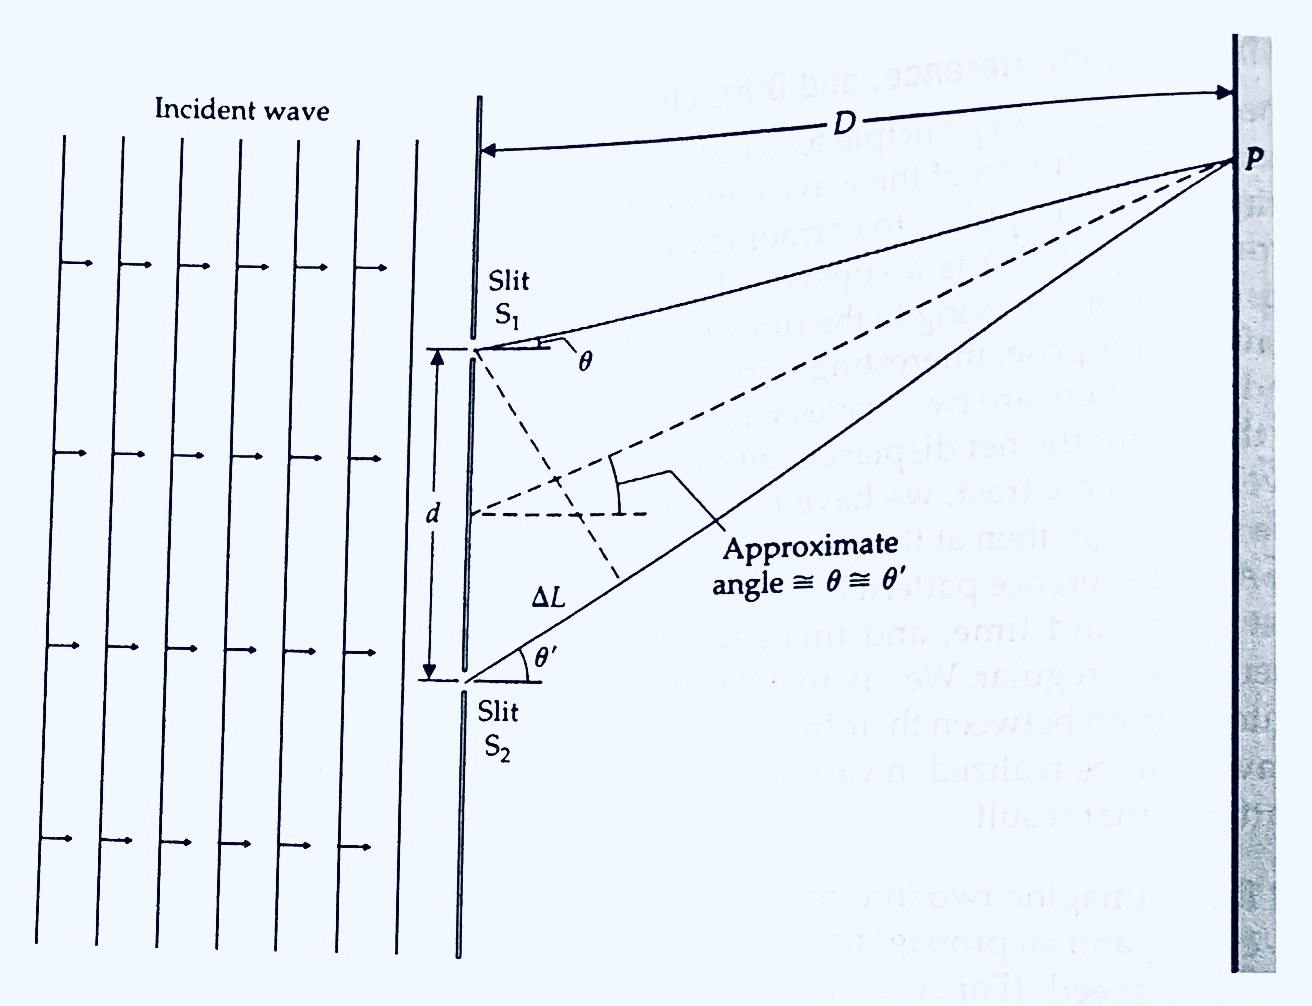
\includegraphics[width=170pt, height=110pt]{interference.jpg}
        \end{center}
        With the setup shown in the figure above, one wave is being split by two slits. $\Delta L$ is the difference in the distance required to travel by each "source". The condition for constructive interference is $\Delta L = n\lambda$; the condition for destructive interference is $\Delta L = (n + 1/2)\lambda$. $n$ is any integer. Using the approximation ($\theta' = \theta$), $\Delta L = d\sin\theta$, so $d\sin\theta = n\lambda$ shows a pattern of constructive interference.
        \newline \indent
        \textbf{Gratings} are similar to the setup shown in the figure except instead of two sources there are $N$ sources to sharpen the interference pattern.
        \newline \indent
        A wave front can also interfere with itself. Wave front propagation can be thought of as a continual regeneration of "waveletes" that interfere with each other to create the straight-line propagation. When there is a barrier, the constructive interference is no longer present so the wave front will bend. This is called \textbf{diffraction}. 
    \subsection*{The Doppler Shift}
        This is how the movement of the receiver or emitter of the wave or medium affects the frequency or wavelength of the wave.